\newpage
\subsubsection{XYZ-Wing}
Bei der Technik \textit{XYZ-Wing} handelt es sich um eine erweiterte Version der Technik \textit{XY-Wing}. Zusätzlich zu den Kandidaten x und y steht hier in der ersten Zelle noch der Kandidat z, der Rest ändert sich nicht. Statt zwei Fällen werden hier drei Fälle betrachtet. Wenn der Kandidat x in der ersten Zelle steht, dann bleibt die Argumentation wie beim \textit{XY-Wing}. Dasselbe gilt für den Fall, dass der Kandidat y in der ersten Zelle steht. Im dritten Fall steht der Kandidat z in der ersten Zelle. In diesem Fall würde er alle Kandidaten ausschließen, die von dort aus direkt auschgeschlossen werden. Daher können alle Kandidaten der Ziffer z gelöscht werden, die von allen drei Zellen ausgeschlossen werden.

\begin{figure}[h]
\begin{center}
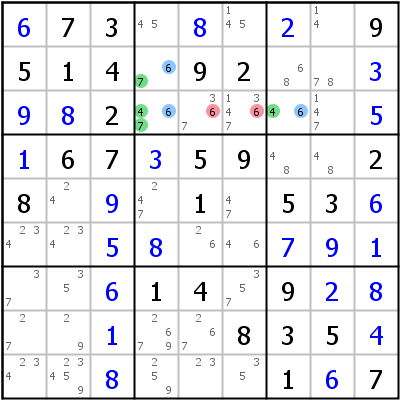
\includegraphics{./img/XYZ_Wing.png}
\caption{XYZ-Wing}
\end{center}
\end{figure}

\noindent In \textbf{Abbildung 2.16} sieht man einen \textit{XYZ-Wing}, dessen erste Zelle z6s1 ist. Hier stehen die Kandidaten 7 für x, 9 für y und 4 für z. Bei z3s1 findet man die zweite Zelle mit den Kandidaten 7 und 4, also x und z. Die dritte Zelle ist z6s2, sie enthält die Kandidaten 9 und 4 und damit y und z. Wir betrachten nun die drei möglichen Fälle für z6s1. Wenn dort die Ziffer 4 steht, dann ist die rot markierte Ziffer 4 in z4s1 direkt ausgeschlossen. Wenn in z6s1 die Ziffer 7 steht, dann kann diese nicht in z3s1 vorkommen, daher muss dort die Ziffer 4 stehen, was diese wiederum in z4s1 ausschließt. Im dritten Fall steht in z6s1 die Ziffer 9, was dazu führt, dass sie nicht in z6s2 stehen kann und daher dort die Ziffer 4 stehen muss. Das schließt auch im letzten möglichen Fall die Ziffer 4 in z4s1 aus, damit kann sie gelöscht werden.